%coding:utf-8

%----------------------------------------
%FOSAPHY, a LaTeX-Code for a summary of linear systems and regulation
%Copyright (C) 2014, Mario Felder, Michael Fallegger

%This program is free software; you can redistribute it and/or
%modify it under the terms of the GNU General Public License
%as published by the Free Software Foundation; either version 2
%of the License, or (at your option) any later version.

%This program is distributed in the hope that it will be useful,
%but WITHOUT ANY WARRANTY; without even the implied warranty of
%MERCHANTABILITY or FITNESS FOR A PARTICULAR PURPOSE.  See the
%GNU General Public License for more details.
%----------------------------------------

\chapter{Regelungstechnik}

\section{Regelkreis}
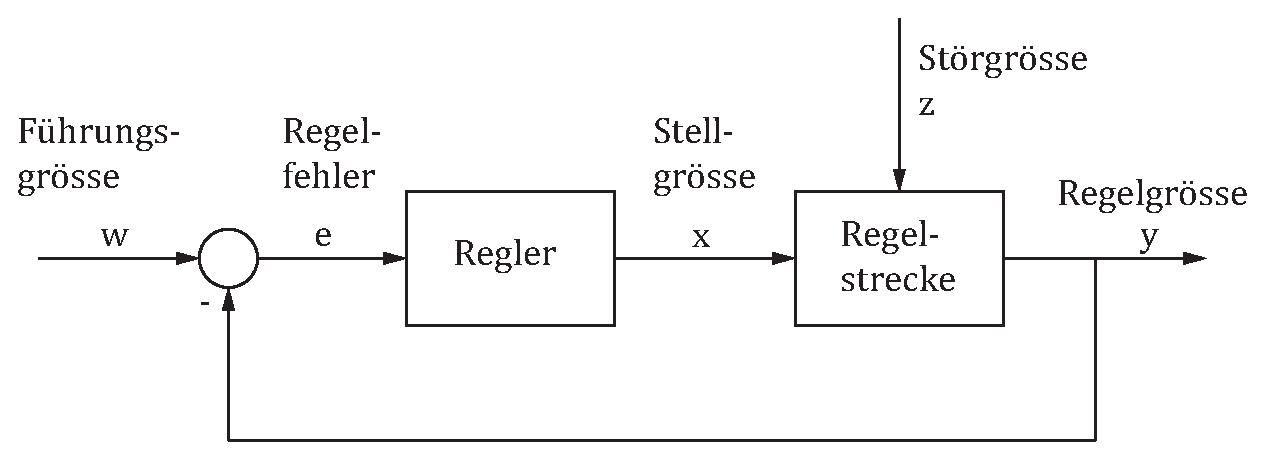
\includegraphics[width = \linewidth]{images/regelkreis.eps}
\\\\
Merkmale:
\begin{itemize}
	\item Erfassen der Regelgrösse $y$
	\item Vergleich von Führungs- und Regelgrösse
	\item Angleichen der Regelgrösse an die Führungsgrösse in Wirkungskreis
\end{itemize}
~\\
Führungsübertragungsverhalten:
\[
	G(s) = \frac{G_R \cdot G_S}{1 + G_R \cdot G_S}
\]
~\\
Störübertragungsverhalten (Störung zwischen Regler und Strecke):
\[
	G_{z1}(s) =\frac{G_S}{1 + G_R \cdot G_S}
\]
~\\
Störübertragungsverhalten (Störung nach Strecke):
\[
	G_{z2}(s) = \frac{1}{1 + G_R \cdot G_S}
\]

\section{Systeme}
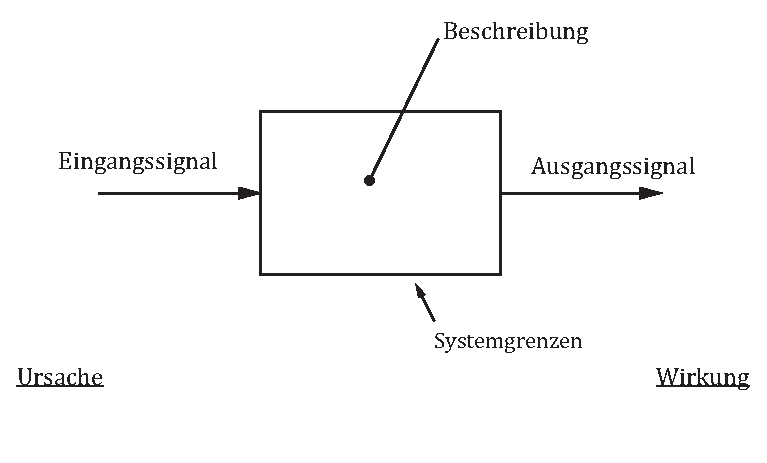
\includegraphics[width = \linewidth]{images/systeme.eps}
\\\\
Signale sind rückwirkungsfrei, also eingeprägte Grössen.
\\\\
\begin{center}
	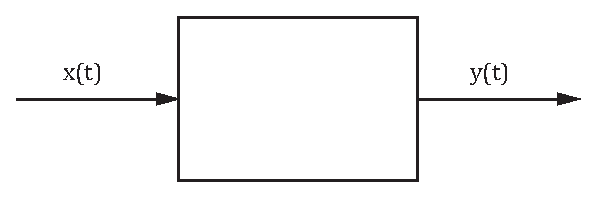
\includegraphics[scale = 0.5]{images/system_bsp.eps}
\end{center}
\newpage

\begin{tabular}{c|l|l}
 Nr. & Bsp & Klassifikation \\ 
\hline 1 & $y(t) = \cos t \cdot x(t)$ & statisch \\ 
	   2 & $\difrac{y(t)}{t} = - \cos (y(t)) + x(t)$ & \textbf{dynamisch} \\ 
\hline 3 & $\difrac{y(t)}{t} = -y(t) + x(t)$ & \textbf{zeitkontinierlich} \\ 
	   4 & $y((k+1)\tau)=-y(k\cdot \tau) + x(k \cdot \tau)$ & zeitdiskret \\ 
\hline 5 & $y(t) = \cos (x (t-\tau))$ & \textbf{kausal} \\ 
 	   6 & $y(t) = \cos(x(t+\tau))$ & nicht kausal \\ 
\hline 7 & $\difrac{y(t)}{t} = -3y(t) + x(t)$ & \textbf{zeitinvariant} \\ 
	   8 & $\difrac{y(t)}{t} = -\cos t \cdot y(t) +x(t)$ & zeitvariant \\ 
\hline 9 & $\difrac{y(t)}{t} = -y(t) +x(t)$ & \textbf{linear} \\ 
	   10 & $\difrac{y(t)}{t} = -y^2(t) +x(t)$ & nicht linear \\ 
\hline 11 & $\difrac{y(t)}{t} = -y(t) +x(t)$ & \textbf{endlich-dimensional} \\ 
	   12 & $\pdifrac{y(t)}{t} = - \pdifrac{}{x}y(x,t)+x(t)$ & unendlich-dimensional \\ 
\hline 13 & $y(t) = t \cdot \cos^2 t \cdot x(t)$ & \textbf{single input/output} \\ 
	   14 & $\left[ \begin{matrix} y_1(t) \\ y_2(t) \end{matrix}\right] = \left[ \begin{matrix} -3 & \sin(t) \\ t & -1\end{matrix}\right] \cdot \left[ \begin{matrix} x_1(t)\\ x_2(t) \end{matrix}\right]$ & multiple input/output \\ 
\end{tabular} 
\\\\

\section{Linearisierung}
Approximation durch Gerade:
\[
	f(\bar{x}+\Delta x) \approx \left.(\bar{x})+\difrac{f}{x}\right|_{\bar{x}}\cdot \Delta x
\]

\subsection{Arbeitspunkt festlegen}

Im stationären Zustand gilt:
\[
	\difrac{^n}{t^n} = 0
\]
~\\
Für das Eingangssignal $u(t)$ und das Ausgangssignal $y(t)$:
\[
	h(t) = \bar{y} + \Delta y(t) \qquad ,\ u(t) = \bar{u} + \Delta u(t)
\]


\subsection{Linearisierung um Arbeitspunkt}
Es gilt:
\[
	D(y^{(n)}, y^{(n-1)}, \dots ,\dot{y} ,y, u^{(m)}, u^{(m-1)}, \dots , \dot{u} ,u)= 0
\]
~\\
$D$ kann am Punkt $\bar{y}, \bar{u}$ approximiert werden durch:
\begin{small}
\[
	\left.\pdifrac{D}{y^{(n)}}\right|_{\begin{scriptsize}\begin{matrix} \bar{y} \\ \bar{u} \end{matrix}\end{scriptsize}} \cdot \Delta y^{n} + \dots +
	\left.\pdifrac{D}{\dot{y}}\right|_{\begin{scriptsize}\begin{matrix} \bar{y} \\ \bar{u} \end{matrix}\end{scriptsize}} \cdot \Delta \dot{y} +
	\left.\pdifrac{D}{y}\right|_{\begin{scriptsize}\begin{matrix} \bar{y} \\ \bar{u} \end{matrix}\end{scriptsize}} \cdot \Delta y +
	\left.\pdifrac{D}{u^{(n)}}\right|_{\begin{scriptsize}\begin{matrix} \bar{y} \\ \bar{u} \end{matrix}\end{scriptsize}} \cdot \Delta u^{n} + \dots +
	\left.\pdifrac{D}{u}\right|_{\begin{scriptsize}\begin{matrix} \bar{y} \\ \bar{u} \end{matrix}\end{scriptsize}} \cdot \Delta u = 0
\]
\end{small}

\begin{center}
	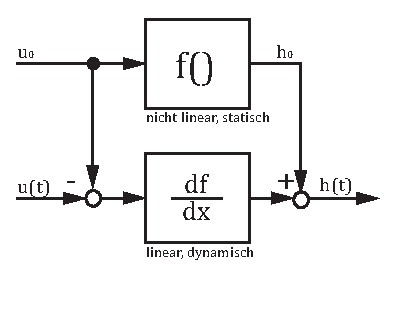
\includegraphics[scale = 0.8]{images/linearisierung.eps}
\end{center}

\section{Stabilität}
Grundlegendes Stabilitätskriterium für LZI-Glieder:\\
\begin{center}
\fbox{\parbox{.9\linewidth}{
	Ein LZI-Glied ist genau dann stabil, wenn die $n$ Nullstellen des Nennerpolynoms sämtliche negative Realteile haben. In der komplexen $s$-Ebene müssen die Nullstellen sämtlich links von der imaginären Achse liegen.
}}
\end{center}

\subsection{Hurwitz-Kriterium}
Das Polynom $N(s) = a_0 + a_1s + a_2s^2 + a_ns^n = 0$ ist nur dann stabil, 
wenn alle Koeffizienten $a_0, a_1, a_2, \ldots a_2$ \uline{ungleich null} sind und
ein \uline{positives Vorzeichen} haben. Zusätzlich müssen alle $n$ \uline{Linieardeterminanten positiv} sein (mit $n$ Zeilen und $n$ Spalten).  
\[
	D_n = \begin{vmatrix}
	a_1 & a_3 & a_5 & a_7 & \ldots \\ 
	a_0 & a_2 & a_4 & a_6 & \ldots \\ 
	0 & a_1 & a_3 & a_5 & \ldots \\ 
	0 & a_0 & a_2 & a_4 & \ldots \\ 
	0 & 0 & a_1 & a_3 & \ldots \\ 
	0 & 0 & a_0 & a_2 & \ldots \\
	\ldots
	\end{vmatrix} 
\]\\
Mit den jeweiligen Unterdeterminanten (für den fall $n=3$):\\
\[\begin{aligned}
	D_1 &= \begin{vmatrix}
		a_1 
		\end{vmatrix} = a_1 > 0\\
	D_2 &= \begin{vmatrix}
		a_1 & a_3 \\
		a_0 & a_2
	\end{vmatrix} = a_1a_2 - a_3a_0 > 0\\
	D_3 &= \begin{vmatrix}
		a_1 & a_3 & 0\\
		a_0 & a_2 & 0\\
		0	& a_1 & a_3
	\end{vmatrix} = a_3 D_2 > 0
\end{aligned}\]\\
Die letzte Determinante erfüllt jeweils zwangsmässig die Bedingung.

\subsection{Nyquist-Kriterium}
Das Stabilitätskriterium nach Nyquist beurteil die Stabilität eines Regelkreises aus dem Velrauf des \textbf{Frequenzgangs des offenen Regelkreises}.
Das Nyquist-Kriterium betrachtet die Ortskurve gegenüber dem Punkt $-1$ auf der reelen Achse. Dabei wird die Winkeländerung von $\omega = 0 \rightarrow \omega = \infty$ betrachtet. Dabei muss folgende Beziehung erfüllt sein, damit das Regelsystem stabil ist:
\[
	\Delta \varphi = i_k \cdot \frac{\pi}{2} + r_k \cdot \pi
\]\\
\begin{footnotesize}
	$r_k$: Anzahl Polstellen mit positivem Realteil\\
	$i_k$: Anzahl Polstellen auf der imaginären Achse
\end{footnotesize}

\begin{center}
	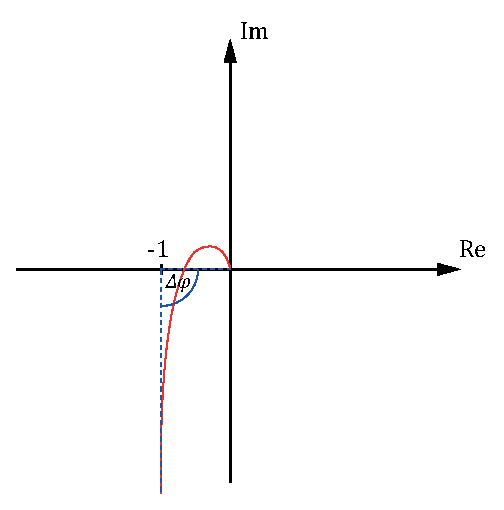
\includegraphics[scale=0.7]{images/nyquist.eps}
\end{center}

\section{Amplituden- und Phasenreserve}
Die Amplitudenreserve $A_R$ ist ein Mass für den Abstand der Ortskurve $G_O(\im\omega)$ vom Punkt $-1$ in Richtung der reelen Achse. Die Kreisfrequenz an der Stelle, an der $G_O(\im\omega)$ die reelle Achse schneidet, heisst Phasenschnittkreisfrequenz $\omega_\pi$.\\
Definition Amplitudenreserve:
\[
	A_R = \frac{1}{\left|G_O(\im\omega_\pi)\right|} \qquad \text{Stabilitätsbedingung: } A_R > 0.
\]\\\\
Die Phasenfrequenz $\varphi_R$ ist der Winkel zwischen der negativ-reellen Achse und dem Punkt, an dem die Ortskurve  $G_O(\im\omega)$ den Einheitskreis schneidet. Die Kreisfrequenz im Schnittpunkt heisst Durchtrittskreisfrequenz $\omega_D$.\\
Definition Phasenreserve:
\[
<<<<<<< HEAD
	\varphi_R = \angle{G_O(\im\omega)} + \pi \qquad \text{Stabilitätsbedingung: } \varphi > 0.
=======
	\varphi_R = \angle{G_O(\im\omega_D)} + \pi \qquad \text{Stabilitätsbedingung: } \varphi > 0.
>>>>>>> 9f5ae5ca8915eff422a188955888ab588b5f3613
\]\\\\
Ablesen von der Ortskurve:
\begin{center}
	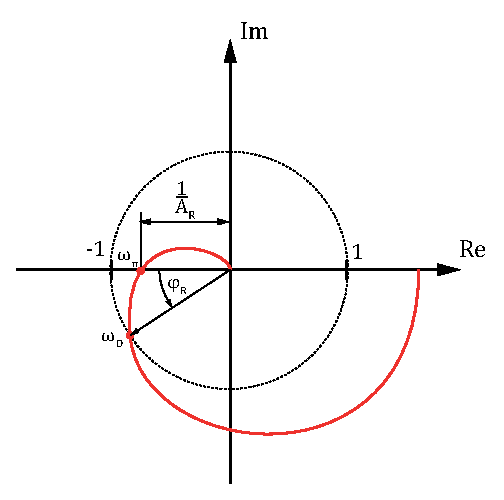
\includegraphics[scale=0.7]{images/ort_reserve.eps}
\end{center}
Ablesen vom Bodediagramm:
\begin{center}
	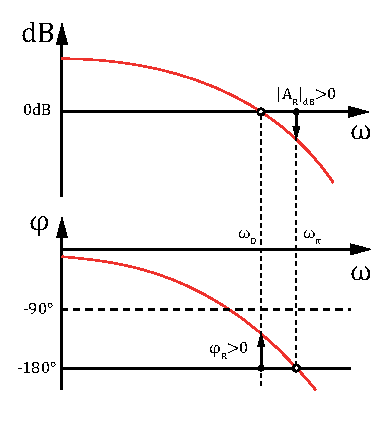
\includegraphics[scale=0.9]{images/bode_reserve.eps}
\end{center}

\subsection{Totzeitreserve}
Die Totzeitreserve $T_{tR}$ ist eine zusätzliche Totzeit, die in einem Regelkreis auftreten darf, ohne dass der Regelkreis instabil wird.\\
Definition Todzeitreserve:
\[
	T_{tR} = \frac{\varphi_R}{\omega_D}
\]
\section{Kompositionen von Grundelementen}

Betrachten der Verkettung:
\begin{center}
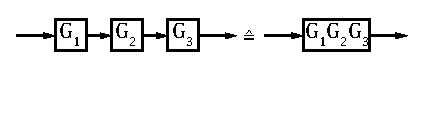
\includegraphics[scale = 1]{images/komp_grnd.eps}
\end{center}
Allgemeine Übertragungsfunktion:
\[
	G(s) = k \frac{s^n \cdot (1+sT_1)^n \ldots}{s^m \cdot (1+sT_2)^m(1+2dTs+s^2T^2)\ldots} \cdot \e^{-sT}
\]
\newpage

\begin{tabular}{>{\centering\arraybackslash}p{1.5cm}|>{\centering\arraybackslash}p{2.5cm}|>{\centering\arraybackslash}p{2cm}|>{\centering\arraybackslash}p{2.5cm}}
	   \rule[-2ex]{0pt}{5.5ex} Anteil  & Bode  & Ortskurve  & Sprungantwort  \\ 
\hline \rule[-2ex]{0pt}{5.5ex} $k$  & 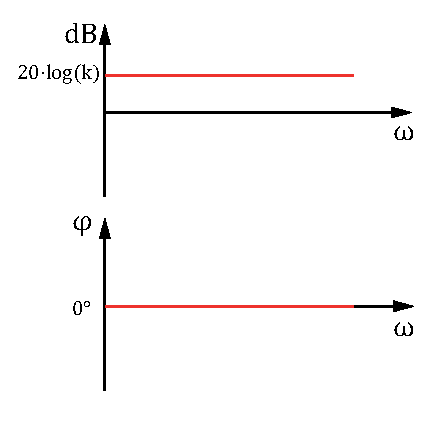
\includegraphics[scale = 0.3]{images/bode_k.eps} & 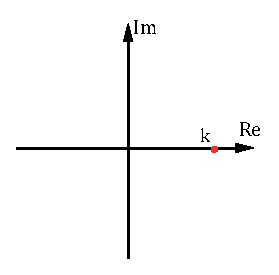
\includegraphics[scale = 0.4]{images/ort_k.eps} & 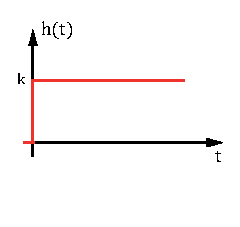
\includegraphics[scale = 0.5]{images/spr_k.eps} \\ 
\hline \rule[-2ex]{0pt}{5.5ex} $s^n$ & 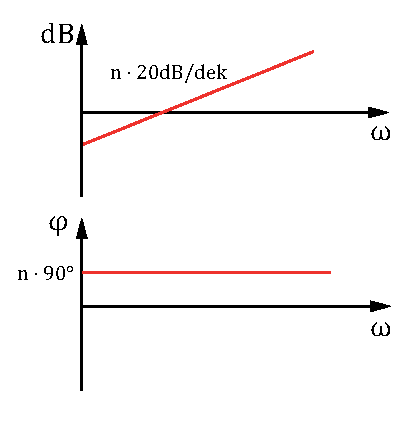
\includegraphics[scale = 0.3]{images/bode_sn.eps} & 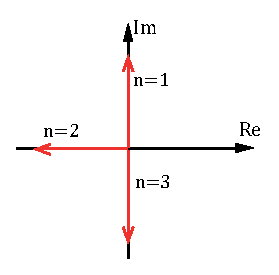
\includegraphics[scale = 0.4]{images/ort_sn.eps}  & 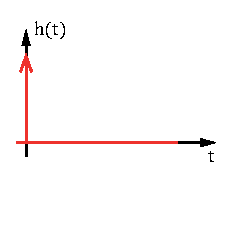
\includegraphics[scale = 0.5]{images/spr_sn.eps}  \\ 
\hline \rule[-2ex]{0pt}{5.5ex} $\frac{1}{s^m}$ & 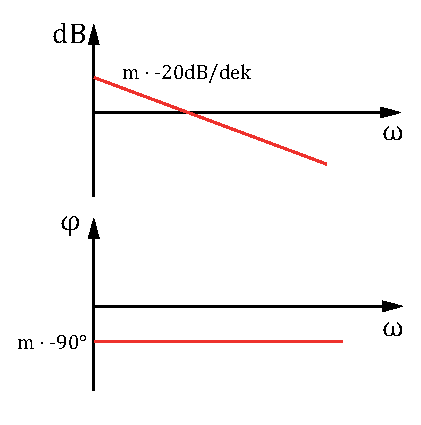
\includegraphics[scale = 0.3]{images/bode_sm.eps}  & 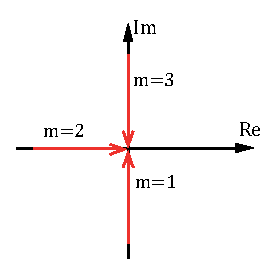
\includegraphics[scale = 0.4]{images/ort_sm.eps}  & 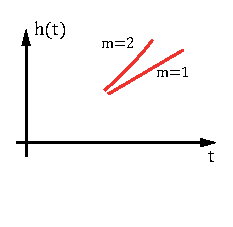
\includegraphics[scale = 0.5]{images/spr_sm.eps} \\ 
\hline \rule[-2ex]{0pt}{5.5ex} $(1+sT)^n$ & 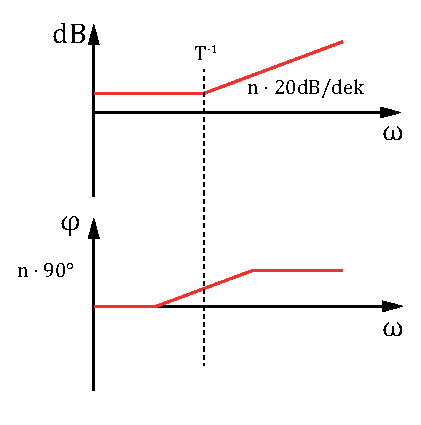
\includegraphics[scale = 0.3]{images/bode_1stn.eps} & 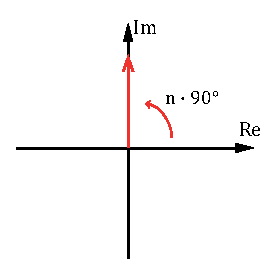
\includegraphics[scale = 0.4]{images/ort_1stn.eps}  & 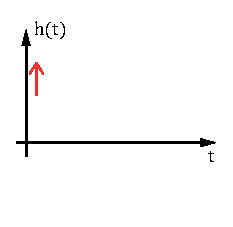
\includegraphics[scale = 0.5]{images/spr_1stn.eps} \\ 
\hline \rule[-2ex]{0pt}{5.5ex} $\frac{1}{(1+sT)^m}$ & 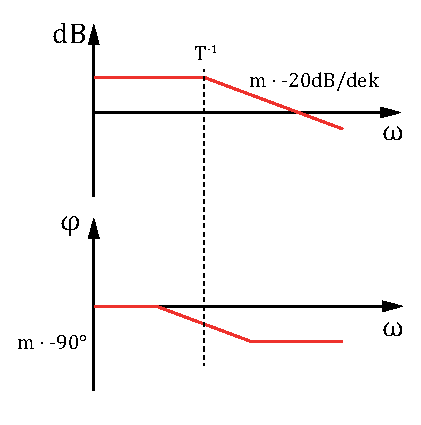
\includegraphics[scale = 0.3]{images/bode_1stm.eps} & 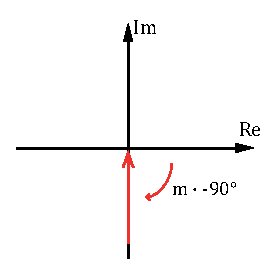
\includegraphics[scale = 0.4]{images/ort_1stm.eps} & 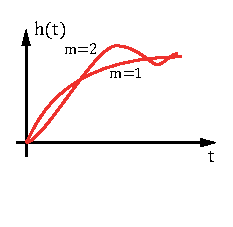
\includegraphics[scale = 0.5]{images/spr_1stm.eps} \\ 
\hline \rule[-2ex]{0pt}{5.5ex} $\e^{-sT}$ & 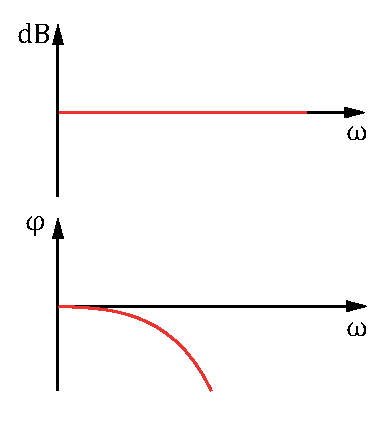
\includegraphics[scale = 0.3]{images/bode_est.eps} & 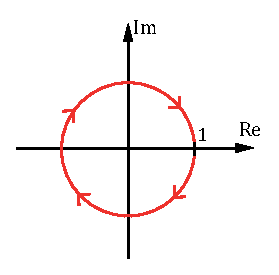
\includegraphics[scale = 0.4]{images/ort_est.eps} & 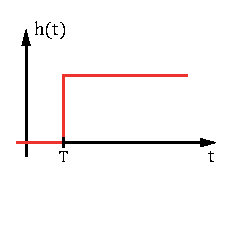
\includegraphics[scale = 0.5]{images/spr_est.eps} \\ 
\end{tabular} 

\section{Stationärer Fehler}
Der stationäre Fehler ist die Differenz zwischen Führungsgrüsse w(t) und Regelgrösse y(t) zum Zeitpunkt $t = \infty$:
\[
	e(\infty) = w(\infty) - y(\infty)
\]
~\\
Diese Grösse kann über den Laplace Endwertsatz berechnet werden:
\[
	 e(\infty) = \lim\limits_{s \rightarrow 0} s \cdot E(s) =  \lim\limits_{s \rightarrow 0} s \cdot \left(W(s) - Y(s)\right)
\]

\newpage

\section{Reglerelemente}
\subsection{Übersicht}
\begin{landscape}\centering
\begin{footnotesize}
\begin{longtable}{|c|c|c|c|c|c|}
\hline Name & $h(t)$ & $G(s)$ & Bode & Ortsk. & PN-Plan \\ 
\hline\endhead $P$ & 
	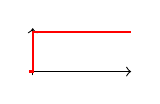
\begin{tikzpicture}[scale=.25]
		\draw[->] (-0.2,0) -- (5,0);
		\draw[->] (0,-0.2) -- (0,2.2);
		\draw[thick, red] (-0.2,0) -- (0,0) -- (0,2) -- (5,2);
	\end{tikzpicture} & $ K_P $ & 
	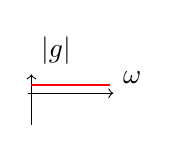
\begin{tikzpicture}[scale=.2]
        \draw[->] (-0.2,0) -- (5.2,0) node[above right] {$\omega$};
        \draw[->] (0,-2) -- (0,1.2) node[above right] {$|g|$};
        \draw[thick, red] (0,0.5) -- (5,0.5);
    \end{tikzpicture}
    \begin{tikzpicture}[scale=.2]
        \draw[->] (-0.2,0) -- (5.2,0) node[above right] {$\omega$};
        \draw[->] (0,-2) -- (0,1.2) node[above right] {$\varphi$};
        \draw[thick, red] (0,0) -- (5,0);
    \end{tikzpicture} & 
    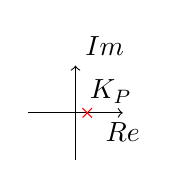
\begin{tikzpicture}[scale=0.3]
         \draw[->] (-2,0) -- (2,0) node[below] {$Re$};
         \draw[->] (0,-2) -- (0,2) node[above right] {$Im$};
         \node[above] at (1.5,0) {$K_P$};
         \draw[red] (.3,0.2) -- (.7,-0.2);
         \draw[red] (.3,-0.2) -- (.7,0.2);
     \end{tikzpicture} & $\nexists$ \\ 
\hline $PT_1$ & 
    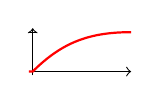
\begin{tikzpicture}[scale=.25]
        \draw[->] (-0.2,0) -- (5,0);
        \draw[->] (0,-0.2) -- (0,2.2);
        \draw[thick, red] (-0.2,0) -- (0,0) to[out=45, in=180] (5,2);
        \draw[-] (-0.2,2) -- (0.2,2);
    \end{tikzpicture} & $\frac{K_P}{1+sT_1}$ & 
    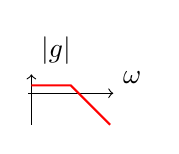
\begin{tikzpicture}[scale=.2]
        \draw[->] (-0.2,0) -- (5.2,0) node[above right] {$\omega$};
        \draw[->] (0,-2) -- (0,1.2) node[above right] {$|g|$};
        \draw[thick, red] (0,0.5) -- (2.5,0.5) -- (5,-2);
    \end{tikzpicture} 
    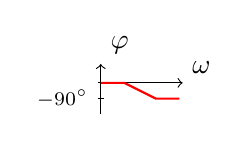
\begin{tikzpicture}[scale=.2]
        \draw[->] (-0.2,0) -- (5.2,0) node[above right] {$\omega$};
        \draw[->] (0,-2) -- (0,1.2) node[above right] {$\varphi$};
        \draw[thick, red] (0,0) -- (1.5,0) -- (3.5,-1) -- (5,-1);
        \draw[-] (-0.2,-1) node[left] {\scriptsize$-90^\circ$} -- (0.2,-1);
    \end{tikzpicture}& 
    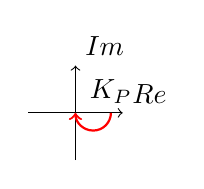
\begin{tikzpicture}[scale=.3]
        \draw[->] (-2,0) -- (2,0) node[above right] {$Re$};
        \draw[->] (0,-2) -- (0,2) node[above right] {$Im$};
        \draw[->, thick, red] (1.5,0) to[out=-90, in=0] (0.75,-0.75) to[out=180,in=-90] (0,0);
        \node[above] at (1.5,0){$K_P$};
    \end{tikzpicture} & 
    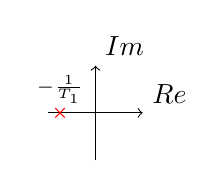
\begin{tikzpicture}[scale=.3]
        \draw[->] (-2,0) -- (2,0) node[above right] {$Re$};
        \draw[->] (0,-2) -- (0,2) node[above right] {$Im$};
        \draw[red] (-1.3,0.2) -- (-1.7,-0.2);
        \draw[red] (-1.3,-0.2) -- (-1.7,0.2);
        \node[above] at (-1.5,0) {\scriptsize$-\frac{1}{T_1}$};
    \end{tikzpicture} \\ 
\hline $PT_2$ & 
    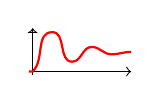
\begin{tikzpicture}[scale=.25]
        \draw[->] (-0.2,0) -- (5,0);
        \draw[->] (0,-0.2) -- (0,2.2);
        \draw[thick, red] (-0.2,0) -- (0,0) to[out=45, in=180] (1,2) to[out=0, in=180] (2,0.5) to[out=0, in=180] (3,1.25) to[out=0, in=180] (4,0.875) to[out=0, in=180] (5,1);
        \draw[-] (-0.2,2) -- (0.2,2);
    \end{tikzpicture} & $\frac{K_P \cdot \omega^2}{{\omega_0}^2 + 2d\omega_0\cdot s + s^2}$ & 
    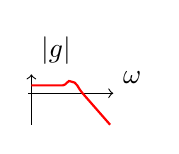
\begin{tikzpicture}[scale=.2]
        \draw[->] (-0.2,0) -- (5.2,0) node[above right] {$\omega$};
        \draw[->] (0,-2) -- (0,1.2) node[above right] {$|g|$};
        \draw[thick, red] (0,0.5) -- (2,0.5) to[out=0 in=180] (2.5,0.75) to[out=0, in=135] (3.25,0) -- (5,-2);
    \end{tikzpicture} 
    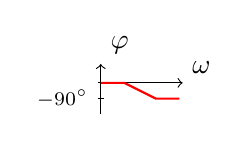
\begin{tikzpicture}[scale=.2]
        \draw[->] (-0.2,0) -- (5.2,0) node[above right] {$\omega$};
        \draw[->] (0,-2) -- (0,1.2) node[above right] {$\varphi$};
        \draw[thick, red] (0,0) -- (1.5,0) -- (3.5,-1) -- (5,-1);
        \draw[-] (-0.2,-1) node[left] {\scriptsize$-90^\circ$} -- (0.2,-1);
    \end{tikzpicture} & 
    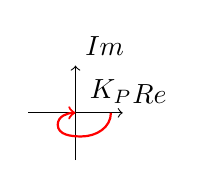
\begin{tikzpicture}[scale=.3]
        \draw[->] (-2,0) -- (2,0) node[above right] {$Re$};
        \draw[->] (0,-2) -- (0,2) node[above right] {$Im$};
        \draw[->, thick, red] (1.5,0) to[out=-90, in=0] (0.25,-1) to[out=180,in=-90] (-.75,-.5) to[out=90, in=180] (0,0);
        \node[above] at (1.5,0){$K_P$};
    \end{tikzpicture} & 
    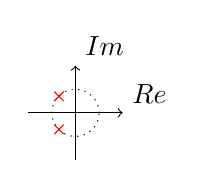
\begin{tikzpicture}[scale=.3]
        \draw[->] (-2,0) -- (2,0) node[above right] {$Re$};
        \draw[->] (0,-2) -- (0,2) node[above right] {$Im$};
        \draw[dotted] (0,0) circle (1);
        \draw[red] (-.5,.5) -- (-.9,.9);
        \draw[red] (-.5,.9) -- (-.9,.5);
        \draw[red] (-.5,-.5) -- (-.9,-.9);
        \draw[red] (-.5,-.9) -- (-.9,-.5);
    \end{tikzpicture} \\ 
\hline $PT_t$ & 
	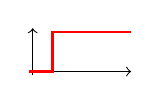
\begin{tikzpicture}[scale=.25]
		\draw[->] (-0.2,0) -- (5,0);
		\draw[->] (0,-0.2) -- (0,2.2);
		\draw[thick, red] (-0.2,0) -- (1,0) -- (1,2) -- (5,2);
	\end{tikzpicture} & $K_P \cdot \e^{-sT_t}$ & 
	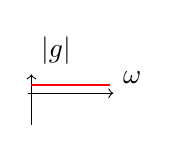
\begin{tikzpicture}[scale=.2]
	     \draw[->] (-0.2,0) -- (5.2,0) node[above right] {$\omega$};
	     \draw[->] (0,-2) -- (0,1.2) node[above right] {$|g|$};
	     \draw[thick, red] (0,0.5) -- (5,0.5);
	 \end{tikzpicture}
	 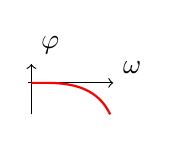
\begin{tikzpicture}[scale=.2]
	     \draw[->] (-0.2,0) -- (5.2,0) node[above right] {$\omega$};
	     \draw[->] (0,-2) -- (0,1.2) node[above right] {$\varphi$};
	     \draw[thick, red] (0,0) -- (1,0) to[out=0, in=115] (5,-2);
	 \end{tikzpicture} & 
	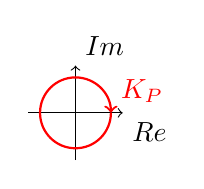
\begin{tikzpicture}[scale=.3]
        \draw[->] (-2,0) -- (2,0) node[below right] {$Re$};
        \draw[->] (0,-2) -- (0,2) node[above right] {$Im$};
        \draw[->, thick, red] (1.5,0) node[above right] {$K_P$} to[out=-90, in=0] (0,-1.5) to[out=180,in=-90] (-1.5,0) to[out=90, in=180] (0,1.5) to[out=0, in=90] (1.5,0);
    \end{tikzpicture} & $\nexists$ \\ 
\hline $D$ & 
    \begin{tikzpicture}[scale=.25]
        \draw[->] (-0.2,0) -- (5,0);
        \draw[->] (0,-0.2) -- (0,2.2);
        \draw[thick, red] (-0.2,0) -- (0,0);
        \draw[->, thick, red] (0,0) -- (0,1.5);
    \end{tikzpicture} & $K_D \cdot s$ & 
    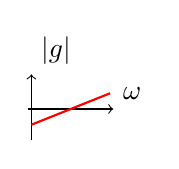
\begin{tikzpicture}[scale=.2]
        \draw[->] (-0.2,0) -- (5.2,0) node[above right] {$\omega$};
        \draw[->] (0,-2) -- (0,2.2) node[above right] {$|g|$};
        \draw[thick, red] (0,-1) -- (5,1);
    \end{tikzpicture}
    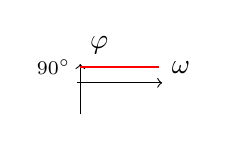
\begin{tikzpicture}[scale=.2]
        \draw[->] (-0.2,0) -- (5.2,0) node[above right] {$\omega$};
        \draw[->] (0,-2) -- (0,1.2) node[above right] {$\varphi$};
        \draw[thick, red] (0,1) -- (5,1);
        \node[left] at (0,1) {\scriptsize$90^\circ$};
    \end{tikzpicture} & 
    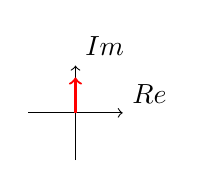
\begin{tikzpicture}[scale=.3]
        \draw[->] (-2,0) -- (2,0) node[above right] {$Re$};
        \draw[->] (0,-2) -- (0,2) node[above right] {$Im$};
        \draw[->, thick, red] (0,0) -- (0,1.5);
    \end{tikzpicture} & 
    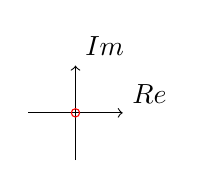
\begin{tikzpicture}[scale=.3]
        \draw[->] (-2,0) -- (2,0) node[above right] {$Re$};
        \draw[->] (0,-2) -- (0,2) node[above right] {$Im$};
        \draw[red] (0,0) circle (5pt);
    \end{tikzpicture} \\ 
\hline $DT_1$ & 
	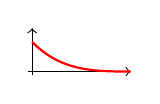
\begin{tikzpicture}[scale=.25]
	  \draw[->] (-0.2,0) -- (5,0);
	  \draw[->] (0,-0.2) -- (0,2.2);
	  \draw[thick, red] (0,1.5) to[out=-45, in=180] (5,0);
	\end{tikzpicture} & $\frac{K_D \cdot s}{1+ sT_1}$ & 
	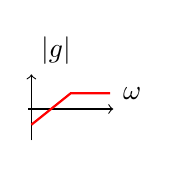
\begin{tikzpicture}[scale=.2]
		\draw[->] (-0.2,0) -- (5.2,0) node[above right] {$\omega$};
		\draw[->] (0,-2) -- (0,2.2) node[above right] {$|g|$};
		\draw[thick, red] (0,-1) -- (2.5,1) -- (5,1);
	\end{tikzpicture}
	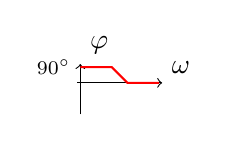
\begin{tikzpicture}[scale=.2]
		\draw[->] (-0.2,0) -- (5.2,0) node[above right] {$\omega$};
		\draw[->] (0,-2) -- (0,1.2) node[above right] {$\varphi$};
		\draw[thick, red] (0,1) -- (2,1) -- (3,0) -- (5,0);
		\node[left] at (0,1) {\scriptsize$90^\circ$};
	\end{tikzpicture} & 
	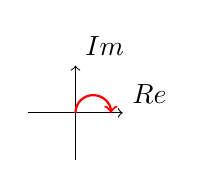
\begin{tikzpicture}[scale=.3]
	   \draw[->] (-2,0) -- (2,0) node[above right] {$Re$};
	   \draw[->] (0,-2) -- (0,2) node[above right] {$Im$};
	   \draw[->, thick, red] (0,0) to[out=90, in=180] (0.75,0.75) to[out=0, in=90] (1.5,0);
	\end{tikzpicture} & 
	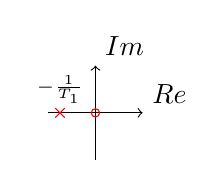
\begin{tikzpicture}[scale=.3]
		\draw[->] (-2,0) -- (2,0) node[above right] {$Re$};
		\draw[->] (0,-2) -- (0,2) node[above right] {$Im$};
		\draw[red] (0,0) circle (5pt);
		\draw[red] (-1.3,0.2) -- (-1.7,-0.2);
		\draw[red] (-1.3,-0.2) -- (-1.7,0.2);
		\node[above] at (-1.5,0) {\scriptsize$-\frac{1}{T_1}$};
	\end{tikzpicture} \\ 
\hline $PD$ & 
    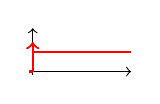
\begin{tikzpicture}[scale=.25]
        \draw[->] (-0.2,0) -- (5,0);
        \draw[->] (0,-0.2) -- (0,2.2);
        \draw[thick, red] (-0.2,0) -- (0,0);
        \draw[->, thick, red] (0,0) -- (0,1.5);
        \draw[thick, red] (0,1) -- (5,1);
    \end{tikzpicture} & $K_p \cdot (1+sT_V)$ & 
	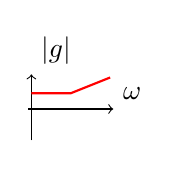
\begin{tikzpicture}[scale=.2]
		\draw[->] (-0.2,0) -- (5.2,0) node[above right] {$\omega$};
		\draw[->] (0,-2) -- (0,2.2) node[above right] {$|g|$};
		\draw[thick, red] (0,1) -- (2.5,1) -- (5,2);
	\end{tikzpicture}
	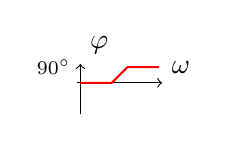
\begin{tikzpicture}[scale=.2]
		\draw[->] (-0.2,0) -- (5.2,0) node[above right] {$\omega$};
		\draw[->] (0,-2) -- (0,1.2) node[above right] {$\varphi$};
		\draw[thick, red] (0,0) -- (2,0) -- (3,1) -- (5,1);
		\node[left] at (0,1) {\scriptsize$90^\circ$};
	\end{tikzpicture} & 
	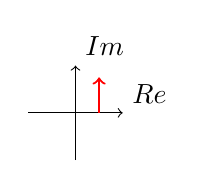
\begin{tikzpicture}[scale=.3]
		\draw[->] (-2,0) -- (2,0) node[above right] {$Re$};
		\draw[->] (0,-2) -- (0,2) node[above right] {$Im$};
		\draw[->, thick, red] (1,0) -- (1,1.5);
	\end{tikzpicture} & 
	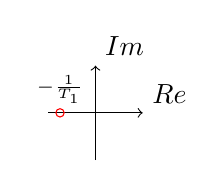
\begin{tikzpicture}[scale=.3]
		\draw[->] (-2,0) -- (2,0) node[above right] {$Re$};
		\draw[->] (0,-2) -- (0,2) node[above right] {$Im$};
		\draw[red] (-1.5,0) circle (5pt);
		\node[above] at (-1.5,0) {\scriptsize$-\frac{1}{T_1}$};
	\end{tikzpicture} \\ 
\hline $PDT_1$ & 
    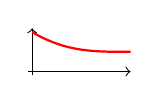
\begin{tikzpicture}[scale=.25]
        \draw[->] (-0.2,0) -- (5,0);
        \draw[->] (0,-0.2) -- (0,2.2);
        \draw[thick, red] (0,2) to[out=-30, in=180] (5,1);
    \end{tikzpicture} & $K_p \cdot \frac{1+T_V}{1+sT_1}$ , $T_V > T_1$ & 
   	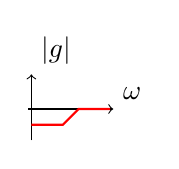
\begin{tikzpicture}[scale=.2]
   		\draw[->] (-0.2,0) -- (5.2,0) node[above right] {$\omega$};
   		\draw[->] (0,-2) -- (0,2.2) node[above right] {$|g|$};
   		\draw[thick, red] (0,-1) -- (2,-1) -- (3,0) -- (5,0);
   	\end{tikzpicture}
   	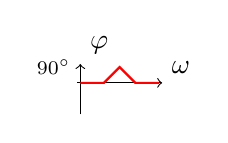
\begin{tikzpicture}[scale=.2]
   		\draw[->] (-0.2,0) -- (5.2,0) node[above right] {$\omega$};
   		\draw[->] (0,-2) -- (0,1.2) node[above right] {$\varphi$};
   		\draw[thick, red] (0,0) -- (1.5,0) -- (2.5,1) -- (3.5,0) -- (5,0);
   		\node[left] at (0,1) {\scriptsize$90^\circ$};
   	\end{tikzpicture} & 
	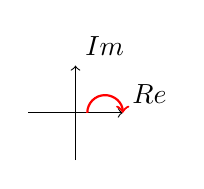
\begin{tikzpicture}[scale=.3]
		\draw[->] (-2,0) -- (2,0) node[above right] {$Re$};
		\draw[->] (0,-2) -- (0,2) node[above right] {$Im$};
		\draw[->, thick, red] (.5,0) to[out=90, in=180] (1.25,.75) to[out=0, in=90] (2,0);
	\end{tikzpicture} & 
	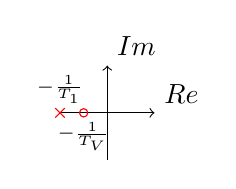
\begin{tikzpicture}[scale=.3]
		\draw[->] (-2,0) -- (2,0) node[above right] {$Re$};
		\draw[->] (0,-2) -- (0,2) node[above right] {$Im$};
		\draw[red] (-1,0) circle (5pt);
		\node[below] at (-1,0) {\scriptsize$-\frac{1}{T_V}$};
		\draw[red] (-2.2,0.2) -- (-1.8,-0.2);
		\draw[red] (-2.2,-0.2) -- (-1.8,0.2);
		\node[above] at (-2,0) {\scriptsize$-\frac{1}{T_1}$};
	\end{tikzpicture} \\ 
\hline $PPT_1$ & 
    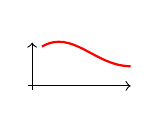
\begin{tikzpicture}[scale=.25]
        \draw[->] (-0.2,0) -- (5,0);
        \draw[->] (0,-0.2) -- (0,2.2);
        \draw[thick, red] (.5,2) to[out=30, in=180] (5,1);
    \end{tikzpicture} & $K_p \cdot \frac{1+T_V}{1+sT_1}$ , $T_V < T_1$ & 
   	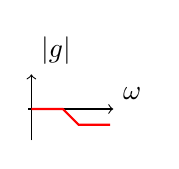
\begin{tikzpicture}[scale=.2]
   		\draw[->] (-0.2,0) -- (5.2,0) node[above right] {$\omega$};
   		\draw[->] (0,-2) -- (0,2.2) node[above right] {$|g|$};
   		\draw[thick, red] (0,0) -- (2,0) -- (3,-1) -- (5,-1);
   	\end{tikzpicture}
   	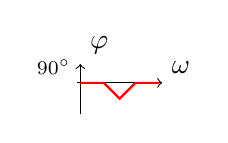
\begin{tikzpicture}[scale=.2]
   		\draw[->] (-0.2,0) -- (5.2,0) node[above right] {$\omega$};
   		\draw[->] (0,-2) -- (0,1.2) node[above right] {$\varphi$};
   		\draw[thick, red] (0,0) -- (1.5,0) -- (2.5,-1) -- (3.5,0) -- (5,0);
   		\node[left] at (0,1) {\scriptsize$90^\circ$};
   	\end{tikzpicture} & 
	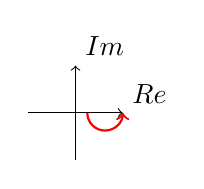
\begin{tikzpicture}[scale=.3]
		\draw[->] (-2,0) -- (2,0) node[above right] {$Re$};
		\draw[->] (0,-2) -- (0,2) node[above right] {$Im$};
		\draw[->, thick, red] (.5,0) to[out=-90, in=180] (1.25,-.75) to[out=0, in=-90] (2,0);
	\end{tikzpicture} & 
	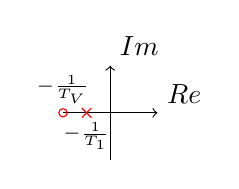
\begin{tikzpicture}[scale=.3]
		\draw[->] (-2,0) -- (2,0) node[above right] {$Re$};
		\draw[->] (0,-2) -- (0,2) node[above right] {$Im$};
		\draw[red] (-2,0) circle (5pt);
		\node[above] at (-2,0) {\scriptsize$-\frac{1}{T_V}$};
		\draw[red] (-1.2,0.2) -- (-.8,-0.2);
		\draw[red] (-1.2,-0.2) -- (-.8,0.2);
		\node[below] at (-1,0) {\scriptsize$-\frac{1}{T_1}$};
	\end{tikzpicture} \\ 
\hline $I$ & 
	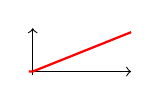
\begin{tikzpicture}[scale=.25]
        \draw[->] (-0.2,0) -- (5,0);
        \draw[->] (0,-0.2) -- (0,2.2);
        \draw[thick, red] (-0.2,0) -- (0,0) -- (5,2);
    \end{tikzpicture} & $K_I \cdot \frac{1}{s}$ & 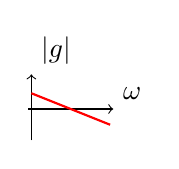
\begin{tikzpicture}[scale=.2]
		\draw[->] (-0.2,0) -- (5.2,0) node[above right] {$\omega$};
		\draw[->] (0,-2) -- (0,2.2) node[above right] {$|g|$};
		\draw[thick, red] (0,1) -- (5,-1);
	\end{tikzpicture}
	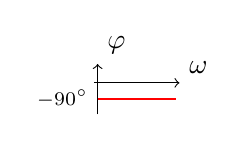
\begin{tikzpicture}[scale=.2]
	    \draw[->] (-0.2,0) -- (5.2,0) node[above right] {$\omega$};
	    \draw[->] (0,-2) -- (0,1.2) node[above right] {$\varphi$};
	    \draw[thick, red] (0,-1) -- (5,-1);
	    \node[left] at (0,-1) {\scriptsize$-90^\circ$};
	\end{tikzpicture} & 
	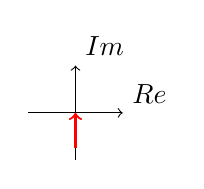
\begin{tikzpicture}[scale=.3]
        \draw[->] (-2,0) -- (2,0) node[above right] {$Re$};
        \draw[->] (0,-2) -- (0,2) node[above right] {$Im$};
        \draw[->, thick, red] (0,-1.5) -- (0,0);
    \end{tikzpicture} & 
    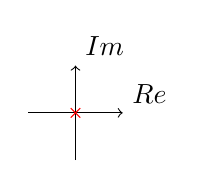
\begin{tikzpicture}[scale=.3]
		\draw[->] (-2,0) -- (2,0) node[above right] {$Re$};
		\draw[->] (0,-2) -- (0,2) node[above right] {$Im$};
		\draw[red] (.2,0.2) -- (-.2,-0.2);
		\draw[red] (.2,-0.2) -- (-.2,0.2);
	\end{tikzpicture} \\ 
\hline $IT_1$ & 
	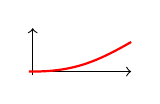
\begin{tikzpicture}[scale=.25]
        \draw[->] (-0.2,0) -- (5,0);
        \draw[->] (0,-0.2) -- (0,2.2);
        \draw[thick, red] (-0.2,0) -- (0,0) to[out=0, in=-150] (5,1.5);
    \end{tikzpicture} & $\frac{K_I}{s \cdot (1+sT_1)}$ & 
	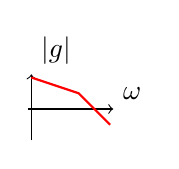
\begin{tikzpicture}[scale=.2]
		\draw[->] (-0.2,0) -- (5.2,0) node[above right] {$\omega$};
		\draw[->] (0,-2) -- (0,2.2) node[above right] {$|g|$};
		\draw[thick, red] (0,2) -- (3,1) -- (5,-1);
	\end{tikzpicture}
	\begin{tikzpicture}[scale=.2]
	    \draw[->] (-0.2,0) -- (5.2,0) node[above right] {$\omega$};
	    \draw[->] (0,-2) -- (0,1.2) node[above right] {$\varphi$};
	    \draw[thick, red] (0,-1) -- (2.5,-1) -- (3.5,-2) -- (5,-2);
	    \node[left] at (0,-1) {\scriptsize$-90^\circ$};
	\end{tikzpicture} & 
	\begin{tikzpicture}[scale=.3]
        \draw[->] (-2,0) -- (2,0) node[above right] {$Re$};
        \draw[->] (0,-2) -- (0,2) node[above right] {$Im$};
        \draw[->, thick, red] (-1,-2) to[out=90, in=180] (0,0);
    \end{tikzpicture} & 
    \begin{tikzpicture}[scale=.3]
		\draw[->] (-2,0) -- (2,0) node[above right] {$Re$};
		\draw[->] (0,-2) -- (0,2) node[above right] {$Im$};
		\draw[red] (.2,0.2) -- (-.2,-0.2);
		\draw[red] (.2,-0.2) -- (-.2,0.2);
		\draw[red] (-1.3,0.2) -- (-1.7,-0.2);
		\draw[red] (-1.3,-0.2) -- (-1.7,0.2);
		\node[above] at (-1.5,0) {\scriptsize$-\frac{1}{T_1}$};
	\end{tikzpicture} \\ 
\hline $PI$ & 
	\begin{tikzpicture}[scale=.25]
        \draw[->] (-0.2,0) -- (5,0);
        \draw[->] (0,-0.2) -- (0,2.2);
        \draw[thick, red] (-0.2,0) -- (0,0) -- (0,1) -- (5,2);
    \end{tikzpicture} & $K_P \cdot \left( 1 + \frac{1}{sT_N} \right)$ & 
	\begin{tikzpicture}[scale=.2]
		\draw[->] (-0.2,0) -- (5.2,0) node[above right] {$\omega$};
		\draw[->] (0,-2) -- (0,2.2) node[above right] {$|g|$};
		\draw[thick, red] (0,2) -- (2.5,1) -- (5,1);
	\end{tikzpicture}
	\begin{tikzpicture}[scale=.2]
	    \draw[->] (-0.2,0) -- (5.2,0) node[above right] {$\omega$};
	    \draw[->] (0,-2) -- (0,1.2) node[above right] {$\varphi$};
	    \draw[thick, red] (0,-1) -- (2,-1) -- (3,0) -- (5,0);
	    \node[left] at (0,-1) {\scriptsize$-90^\circ$};
	\end{tikzpicture} & 
	\begin{tikzpicture}[scale=.3]
        \draw[->] (-2,0) -- (2,0) node[above right] {$Re$};
        \draw[->] (0,-2) -- (0,2) node[above right] {$Im$};
        \draw[->, thick, red] (1,-2) -- (1,0);
    \end{tikzpicture} & 
	\begin{tikzpicture}[scale=.3]
		\draw[->] (-2,0) -- (2,0) node[above right] {$Re$};
		\draw[->] (0,-2) -- (0,2) node[above right] {$Im$};
		\draw[red] (.2,0.2) -- (-.2,-0.2);
		\draw[red] (.2,-0.2) -- (-.2,0.2);
		\draw[red] (-1.5,0) circle (5pt);
		\node[above] at (-1.5,0) {\scriptsize$-\frac{1}{T_1}$};
	\end{tikzpicture} \\ 
\hline $PID$ & 
	\begin{tikzpicture}[scale=.25]
        \draw[->] (-0.2,0) -- (5,0);
        \draw[->] (0,-0.2) -- (0,2.2);
        \draw[thick, red] (0,2) -- (0,1) -- (5,2);
    \end{tikzpicture} & $K_P \cdot \left( 1 + \frac{1}{sT_N} +sT_V \right)$ & 
	\begin{tikzpicture}[scale=.2]
		\draw[->] (-0.2,0) -- (5.2,0) node[above right] {$\omega$};
		\draw[->] (0,-2) -- (0,2.2) node[above right] {$|g|$};
		\draw[thick, red] (0,2) -- (2,1) -- (3,1) -- (5,2);
	\end{tikzpicture}
	\begin{tikzpicture}[scale=.2]
	    \draw[->] (-0.2,0) -- (5.2,0) node[above right] {$\omega$};
	    \draw[->] (0,-2) -- (0,1.2) node[above right] {$\varphi$};
	    \draw[thick, red] (0,-1) -- (1.5,-1) -- (3.5,1) -- (5,1);
	    \node[left] at (0,-1) {\scriptsize$-90^\circ$};
	\end{tikzpicture} & 
	\begin{tikzpicture}[scale=.3]
		\draw[->] (-2,0) -- (2,0) node[above right] {$Re$};
		\draw[->] (0,-2) -- (0,2) node[above right] {$Im$};
		\draw[->, thick, red] (1,-2) -- (1,2);
	\end{tikzpicture} & 
	\begin{tikzpicture}[scale=.3]
		\draw[->] (-2,0) -- (2,0) node[above right] {$Re$};
		\draw[->] (0,-2) -- (0,2) node[above right] {$Im$};
		\draw[red] (.2,0.2) -- (-.2,-0.2);
		\draw[red] (.2,-0.2) -- (-.2,0.2);
		\draw[red] (-1.5,0) circle (5pt);
		\draw[red] (-.75,0) circle (5pt);
	\end{tikzpicture} \\ 
\hline $PIDT_1$ & 
	\begin{tikzpicture}[scale=.25]
        \draw[->] (-0.2,0) -- (5,0);
        \draw[->] (0,-0.2) -- (0,2.2);
        \draw[thick, red] (0,2) to[out=-60, in=150] (0.75,1) to[out=-30, in=190] (2.5,1)-- (5,1.5);
    \end{tikzpicture} & $K_P \cdot \left( 1 + \frac{1}{sT_N} + \frac{sT_V}{1+sT_1} \right)$ & 
	\begin{tikzpicture}[scale=.2]
		\draw[->] (-0.2,0) -- (5.2,0) node[above right] {$\omega$};
		\draw[->] (0,-2) -- (0,2.2) node[above right] {$|g|$};
		\draw[thick, red] (0,2) -- (1,1) -- (2,1) -- (3,1.5) -- (5,1.5);
	\end{tikzpicture}
	\begin{tikzpicture}[scale=.2]
	    \draw[->] (-0.2,0) -- (5.2,0) node[above right] {$\omega$};
	    \draw[->] (0,-2) -- (0,1.2) node[above right] {$\varphi$};
	    \draw[thick, red] (0,-1) -- (.5,-1) -- (2.5,1) -- (3.5,0) -- (5,0);
	    \node[left] at (0,-1) {\scriptsize$-90^\circ$};
	    \node[left] at (0,1) {\scriptsize$90^\circ$};
	\end{tikzpicture} & 
	\begin{tikzpicture}[scale=.3]
		\draw[->] (-2,0) -- (2,0) node[above right] {$Re$};
		\draw[->] (0,-2) -- (0,2) node[above right] {$Im$};
		\draw[->, thick, red] (.5,-2) -- (.5,0) to[out=90, in=180] (1.25,0.75) to[out=0, in=90] (2,0);
	\end{tikzpicture} & 
	\begin{tikzpicture}[scale=.3]
		\draw[->] (-2,0) -- (2,0) node[above right] {$Re$};
		\draw[->] (0,-2) -- (0,2) node[above right] {$Im$};
		\draw[red] (.2,0.2) -- (-.2,-0.2);
		\draw[red] (.2,-0.2) -- (-.2,0.2);
		\draw[red] (-1.5,0) circle (5pt);
		\draw[red] (-.75,0) circle (5pt);
		\draw[red] (-2.2,0.2) -- (-1.8,-0.2);
		\draw[red] (-2.2,-0.2) -- (-1.8,0.2);
	\end{tikzpicture} \\ 
\hline 
\end{longtable} 
\end{footnotesize}
\end{landscape}
\clearpage

\subsection{$P$-Glied}
\begin{tabular}{ll}
\rule[-2ex]{0pt}{5.5ex} DGL: & $y(t) = K_P \cdot w(t)$ \\ 
\rule[-2ex]{0pt}{5.5ex} Übertragungsfunktion: & $G(s) = K_P$ \\ 
\rule[-2ex]{0pt}{5.5ex} Sprungantwort: & $h(t) = K_P$ \\ 
\end{tabular} 
\subsection{$PT_1$-Glied}
\begin{tabular}{ll}
\rule[-2ex]{0pt}{5.5ex} DGL: &  $T_1 \cdot \dot{y}(t) + y(t) = K_p \cdot u(t)$\\ 
\rule[-2ex]{0pt}{5.5ex} Übertragungsfunktion: & $G(s) = K_P$ \\ 
\rule[-2ex]{0pt}{5.5ex} Sprungantwort: & $h(t) = K_P$ \\ 
\end{tabular} 
\subsection{$PT_2$-Glied}
\begin{tabular}{ll}
\rule[-2ex]{0pt}{5.5ex} DGL: & $\ddot{y}(t) + 2d\omega\cdot \dot{y}(t)+y=K_p \cdot u(t)$ \\ 
\rule[-2ex]{0pt}{5.5ex} Übertragungsfunktion: & $G(s) = K_P$ \\ 
\rule[-2ex]{0pt}{5.5ex} Sprungantwort: & $h(t) = K_P$ \\ 
\end{tabular} 
\subsection{$PT_t$-Glied}
\begin{tabular}{ll}
\rule[-2ex]{0pt}{5.5ex} DGL: & $y(t) = K_p \cdot u(t-T_t)$ \\ 
\rule[-2ex]{0pt}{5.5ex} Übertragungsfunktion: & $G(s) = K_P$ \\ 
\rule[-2ex]{0pt}{5.5ex} Sprungantwort: & $h(t) = K_P$ \\ 
\end{tabular} 
\subsection{$D$-Glied}
\begin{tabular}{ll}
\rule[-2ex]{0pt}{5.5ex} DGL: & $y(t) = K_D \cdot \dot{u}(t)$ \\ 
\rule[-2ex]{0pt}{5.5ex} Übertragungsfunktion: & $G(s) = K_P$ \\ 
\rule[-2ex]{0pt}{5.5ex} Sprungantwort: & $h(t) = K_P$ \\ 
\end{tabular} 
\subsection{$DT_1$-Glied}
\begin{tabular}{ll}
\rule[-2ex]{0pt}{5.5ex} DGL: & $T_1 \cdot \dot{y}(t) + y(t) = K_D \cdot \dot{u}(t)$ \\ 
\rule[-2ex]{0pt}{5.5ex} Übertragungsfunktion: & $G(s) = K_P$ \\ 
\rule[-2ex]{0pt}{5.5ex} Sprungantwort: & $h(t) = K_P$ \\ 
\end{tabular} 
\subsection{$PD$-Glied}
\begin{tabular}{ll}
\rule[-2ex]{0pt}{5.5ex} DGL: & $y(t) = K_p \cdot \left(T_V \cdot \dot{u}(t) + u(t)\right)$ \\ 
\rule[-2ex]{0pt}{5.5ex} Übertragungsfunktion: & $G(s) = K_P$ \\ 
\rule[-2ex]{0pt}{5.5ex} Sprungantwort: & $h(t) = K_P$ \\ 
\end{tabular} 
\subsection{$PDT_1$-Glied}
\begin{tabular}{ll}
\rule[-2ex]{0pt}{5.5ex} DGL: & $T_1 \dot{y}(t) + y(t) = K_p \cdot \left( T_V \cdot \dot{u}(t) + u(t)\right)$ , $T_V > T_1$ \\ 
\rule[-2ex]{0pt}{5.5ex} Übertragungsfunktion: & $G(s) = K_P$ \\ 
\rule[-2ex]{0pt}{5.5ex} Sprungantwort: & $h(t) = K_P$ \\ 
\end{tabular} \\
\subsection{$PPT_1$-Glied}
\begin{tabular}{ll}
\rule[-2ex]{0pt}{5.5ex} DGL: & $T_1 \dot{y}(t) + y(t) = K_p \cdot \left( T_V \cdot \dot{u}(t) + u(t)\right)$ , $T_V < T_1$ \\ 
\rule[-2ex]{0pt}{5.5ex} Übertragungsfunktion: & $G(s) = K_P$ \\ 
\rule[-2ex]{0pt}{5.5ex} Sprungantwort: & $h(t) = K_P$ \\ 
\end{tabular} 
\subsection{$I$-Glied}
\begin{tabular}{ll}
\rule[-2ex]{0pt}{5.5ex} DGL: & $\dot{y} = K_I u(t)$ \\ 
\rule[-2ex]{0pt}{5.5ex} Übertragungsfunktion: & $G(s) = K_P$ \\ 
\rule[-2ex]{0pt}{5.5ex} Sprungantwort: & $h(t) = K_P$ \\ 
\end{tabular} 
\subsection{$IT_1$-Glied}
\begin{tabular}{ll}
\rule[-2ex]{0pt}{5.5ex} DGL: & $T_1 \cdot \ddot{y}(t) + \dot{y}(t) = K_I \cdot u(t)$ \\ 
\rule[-2ex]{0pt}{5.5ex} Übertragungsfunktion: & $G(s) = K_P$ \\ 
\rule[-2ex]{0pt}{5.5ex} Sprungantwort: & $h(t) = K_P$ \\ 
\end{tabular} 
\subsection{$PI$-Glied}
\begin{tabular}{ll}
\rule[-2ex]{0pt}{5.5ex} DGL: & $y(t) = K_P \cdot \left( u(t) + \frac{1}{T_N}\int u(t) \di t\right)$ \\ 
\rule[-2ex]{0pt}{5.5ex} Übertragungsfunktion: & $G(s) = K_P$ \\ 
\rule[-2ex]{0pt}{5.5ex} Sprungantwort: & $h(t) = K_P$ \\ 
\end{tabular} 
\subsection{$PID$-Glied}
\begin{tabular}{ll}
\rule[-2ex]{0pt}{5.5ex} DGL: &  $y(t) = K_P \cdot \left( u(t) + \frac{1}{T_N}\int u(t) \di t + T_V \cdot \dot{u}(t) \right)$ \\ 
\rule[-2ex]{0pt}{5.5ex} Übertragungsfunktion: & $G(s) = K_P$ \\ 
\rule[-2ex]{0pt}{5.5ex} Sprungantwort: & $h(t) = K_P$ \\ 
\end{tabular} 
\subsection{$PIDT_1$-Glied}
\begin{tabular}{ll}
\rule[-2ex]{0pt}{5.5ex} DGL: & \scriptsize$T_1 \cdot \dot{y}(t) +y(t) = K_P \cdot \left( \frac{T_1 + T_N}{T_N} u(t) + \frac{1}{T_N}\int u(t) \di t + (T_1 + T_V) \cdot \dot{u}(t) \right)$ \\ 
\rule[-2ex]{0pt}{5.5ex} Übertragungsfunktion: & $G(s) = K_P$ \\ 
\rule[-2ex]{0pt}{5.5ex} Sprungantwort: & $h(t) = K_P$ \\ 
\end{tabular}
